%!TEX root = ../../../../report.tex

\subsection{Ankle and knee joint mechanics} % (fold)
\label{sub:hip_and_knee_joint_mechanics}
Several mechanical configurations were sketched as the first step of the iterations in the mechanical design of the joints.
As previously explained, the hip joint turned out to have lower design constraints, since belt and compliance were not required, although the use of gears was a need.
However, for the knee and ankle joints, the need of integrated compliance and the torque transmission through a pulley yielded some restrictions that resulted in a final configuration as in \ref{fig:knee_joint}.

\begin{figure}[htb]
  \centering
  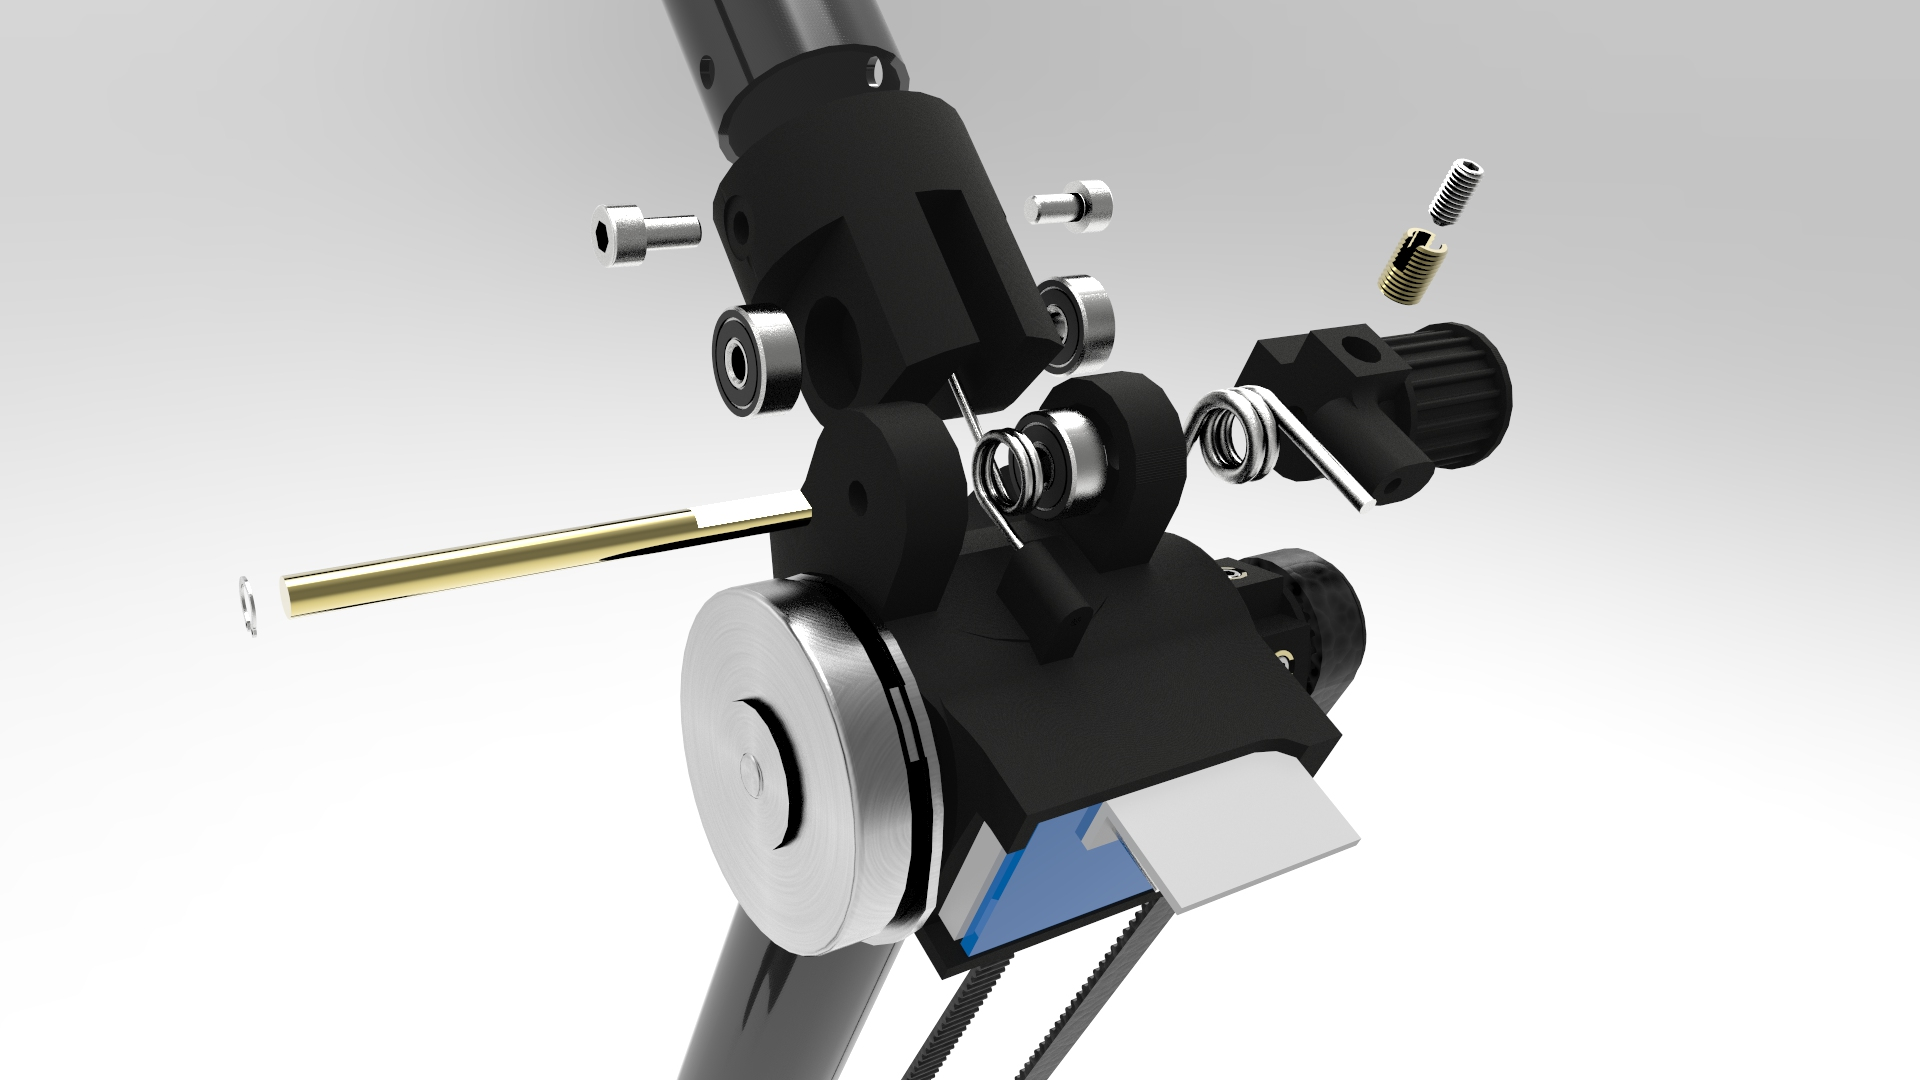
\includegraphics[width=\textwidth]{figures/legs_knee_deconstructed.jpg}
  \caption{Knee joint mechanical implementation.}
  \label{fig:knee_joint}
\end{figure}

The configuration in \ref{fig:knee_joint} is equivalent for the ankles.
Therefore, four bearings, a rod and the interfaces for the springs are needed and thus, discussed below.

\subsubsection{Joints axes} % (fold)
\label{ssub:rods}
The characteristics of the rod used as axis of the angular motion of the joint are studied here.
It is also used, in the case of the knee and the ankle, as a support for the pulleys that transmit the power from the motor to the next link.
Three mechanical efforts bound its design:
\begin{enumerate}
  \item \textbf{Shear effort}: produced when an impact occurs and the internal efforts are transmitted through the rod between the two links that form the joint.
  \item \textbf{Bending effort}: caused by the perpendicular force created by belt in tension on the edge of the rod.
  \item \textbf{Torsion effort}: due to the pulley in the knee and the ankle. 
  This effort is negligible because zero-friction bearings are supposed.
\end{enumerate}

  \paragraph{Shear analysis} % (fold)
  \label{ssub:shear_analysis}
  The maximum shear stress is found in the diameter of the cylinder (y=0) and is:
  
  \noindent\begin{minipage}{0.2\textwidth}% adapt widths of minipages to your needs
  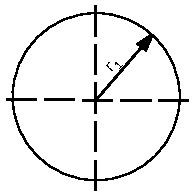
\includegraphics[width=\linewidth]{figures/profile_tube.pdf}
  \end{minipage}%
  \hfill%
  \begin{minipage}{0.8\textwidth}
    \begin{equation}
    \begin{aligned}
      \gamma_{yz} &= \frac{Q_y M_{x}^A*}{b(y) I_x} = \frac{Q}{r^2}\\
      M_{x}^{A_{y=0}} &= \frac{\pi r_1^2}{2} \\
      b(y=0) &= 2 r_1 \\
      I_x &= \frac{\pi r_1^4}{4}
      \end{aligned}
    \end{equation}
  \end{minipage}
  Given a tangent force Q, the shear stress can be calculated.
  If this is over the ultimate strength, the cylinder will break.
  % paragraph shear_analysis (end)

  \paragraph{Bending} % (fold)
  \label{ssub:bending}
  The bending analysis follows the one carried out in the section \ref{ssub:profile_study} for a cylinder.
  The equivalent force in this case is given by the tension of the belts, mainly the initial (though there are other tensions that appear when the belts moves for example).
  Due to feasibility reasons and the lack of the appropriate measurements devices, some experimental tests trying different tensions and axes where carried out giving good results with a 3 mm rod or more.
  % paragraph bending (end)

  \paragraph{Sizing} % (fold)
  \label{ssub:sizing}
  The studies above have been tested for different diameters of rod starting from the smallest size given by the provider and increasing until both conditions are satisfied, due to the requirements of weight reduction.
  In case of using steel as material, the ultimate strength is supposed to be 250 MPa \footnote{https://en.wikipedia.org/wiki/A36\_steel}.
  And for the case of a rod of 3 mm of diameter, both stress efforts are under the resulting restrictions.
  Thus, 3 mm rods were selected for both ankles and knees.
  % paragraph sizing (end)
% subsubsection rods (end)

\subsubsection{Bearings on the joints} % (fold)
\label{ssub:bearings}
The force calculated in section \ref{sub:impact_force} has been used for sizing the bearings of the knee and the ankle.
The bearing selected should be such that allowed dynamic loads of more than the impact force while being as small as possible to reduce additional weight on the frame.
Besides, their internal diameter is defined by the rod diameter calculated in section \ref{ssub:rods}.

An estimation of nominal life of the bearing can be done from the Dynamic Load Rating (C), the Dynamic Equivalent Load (P) and the Life Rime Coefficient for a Ball Bearing (p) (being p=3 for balls bearings).
Equation \ref{eq:service_life_bearing} shows the nominal life of a ball bearing, which can be used in order to calculate the nominal life for a specific application.
It is also worth mentioning that the Dynamic Equivalent Load (P) is divided by the number of bearings in which the force is spread.
\begin{equation}
  \label{eq:service_life_bearing}
  L_{10} = \frac{10^{6}}{60 n} \left(\frac{C}{P}\right)^{p}
\end{equation}

The term $L$ is the service life of a bearing (in number of hours or rpm), in normal conditions of speed and load, in which the bearing is working until fail by fatigue. 
Whilst $L_{10}$ is based in a statistical model that is defined as the 90\% of the bearing of the same type will withstand those loads for a longer time.
% subsubsection bearings (end)

\subsubsection{Springs dimensions} % (fold)
\label{ssub:springs_dimensions}
A big set of springs have been ordered in order to include them to the toolkit provided for experimentation, so that the trials detailed in \ref{ssub:experiment_2} can be conducted.
The criteria for the selection of the springs have been torsion model and 90\degree angle, ordering a left and right model of each since the mechanical interfaces on the robot are mirrored.
Any of the acquired springs can be placed in any holder since the holes for inserting them have been designed with the diameter of the biggest one ordered plus a small clearance obtained from \ref{sub:arc_compensation}.

Exact calculation to obtain the stiffness of springs used for adding compliance to the joints of a legged machine have not been found in the literature. 
For research in a specific kind of gait, at a determined speed, the usual solution is to study real individuals and collect data from their analysis or empirically optimize the values through recurrent iterations until a good value is found.
However, the fact that RuBi is not meant to be optimized for a determined speed or gait, but it is supposed to work in a wide range, prevented from conducting this kind of studies.
Thus, the final values of stiffness were theoretically inferred from an adapted average of the implemented values for ankles in \cite{grimmer}.
They correspond to the values of $K$ in the middle of the range ordered.
A list of the purchased springs can be found in appendix \ref{sec:available_springs_}.
The stiffest models have been selected to ensure the rigid behavior needed to implement a direct drive configuration in the actuation through a rough estimation of maximum torque requirements.
Besides, the use of longer axes in the joints would allow the combination of springs in series for the SEA configuration, increasing the actual range of available values of $K$.
This is suggested here as further work.


% subsubsection springs_dimensions (end)

\subsubsection{Implementation of elastic actuation} % (fold)
\label{ssub:spring_integration}
In section \ref{sec:joints} the use of springs is justified in order to walk and run efficiently. 
An analysis of the different possibilities to include compliance in the robot is done in the same section, while Figure \ref{fig:compliance_series} shows the analyzed configurations and their advantages and disadvantages are further discussed.
The final design has been conceived to allow for any of the four possible springs configurations shown in Figure \ref{fig:pasive_actuators} to be implemented in the knee and ankle joints.
This is possible by making a system that allows to put elastic components in series and parallel that are easily replaceable.

\paragraph{SEA configuration} % (fold)
\label{para:sea_configuration}

In the section commented above, it is also determined the use of rotational springs for both series and parallel passive actuators.
This gives a more constrained design that is later used as a feature.
For example, in the section \ref{sub:pulleys_and_belts} is explained how the the pulley is integrated in a part that has the task of both being the place to put the spring and being the pulley.
The Figure \ref{fig:serial_spring_pulley} shows this.
This design shows the implementation of the SEA configurations that can be adjusted by changing the physical properties of the spring.
% paragraph sea_configuration (end)

\paragraph{PEA configuration} % (fold)
\label{para:pea_configuration}

The parallel spring is implemented by adding a spring directly attached to both links of the joint.
The problem of the parallel passive actuators is the need of loading the spring for movements in which is maybe not appropriated.
As an example, the rest position of the parallel spring in the ankle could be placed when the foot is at 90 degrees with its consecutive link, so the robot can be stood up without applying any extra torque in the motors to keep balance.
This would mean though to do an extra effort against the spring when taking off.
In the same line of giving all the possibilities to the user with the compliance, a system that allows to change the rest position of the parallel spring has been implemented.
This consists of one arm of the torsional spring attached to one of the links of the joint while the other arm can be fastened in different relative angles.
The Figure \ref{fig:rotational_spring_rest_position} shows the transversal section of the joint component where the parallel spring can adopt different configurations. 

The above explained design allows to implement a PEA configuration on the joints by just adding a spring and using an overdimensioned spring for the transmission from the pulley that can act as a DD.

\begin{figure}[ht!]
  \centering
  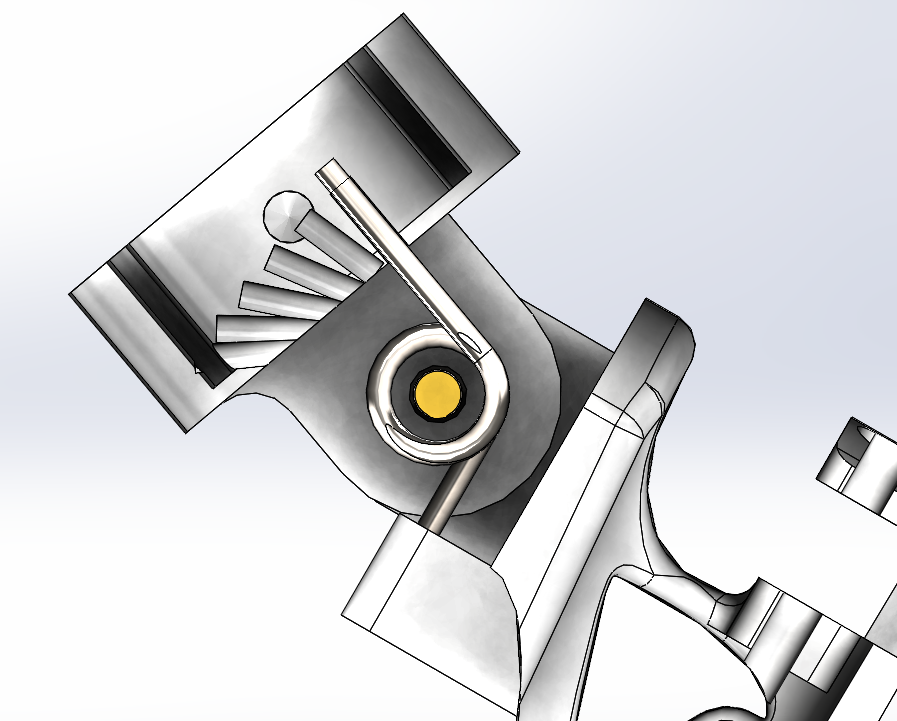
\includegraphics[width=0.75\textwidth]{figures/rotational_spring_rest_positions}
  \caption{Transversal section of the parallel spring resting positions in the left ankle.}
  \label{fig:rotational_spring_rest_position}
\end{figure}
% paragraph pea_configuration (end)

\paragraph{SEA + PEA configuration} % (fold)
\label{ssub:sea_pea_configuration}
The possibility of using both, SEA and PEA, configurations at the same time is offered.
This allows for the study of the SEA+PEA combination.
% paragraph sea_pea_configuration (end)

\paragraph{DD configuration } % (fold)
\label{ssub:dd_configuration}
Finally if no parallel spring is used and a spring stiff enough that does not add compliance to the system is placed in the SEA configuration, a DD transmission is achieved.
% paragraph dd_configuration (end)

% subsubsection spring_integration (end)

% subsection hip_and_knee_joint_mechanics (end)
